% RFG-R figure block.
% Place this file beside main.tex. It expects the directory
% r_universe_completion/generated/figures/ beside it as well.
% Requires: \usepackage{graphicx} and \usepackage{float}.

\begin{figure}[H]
\centering
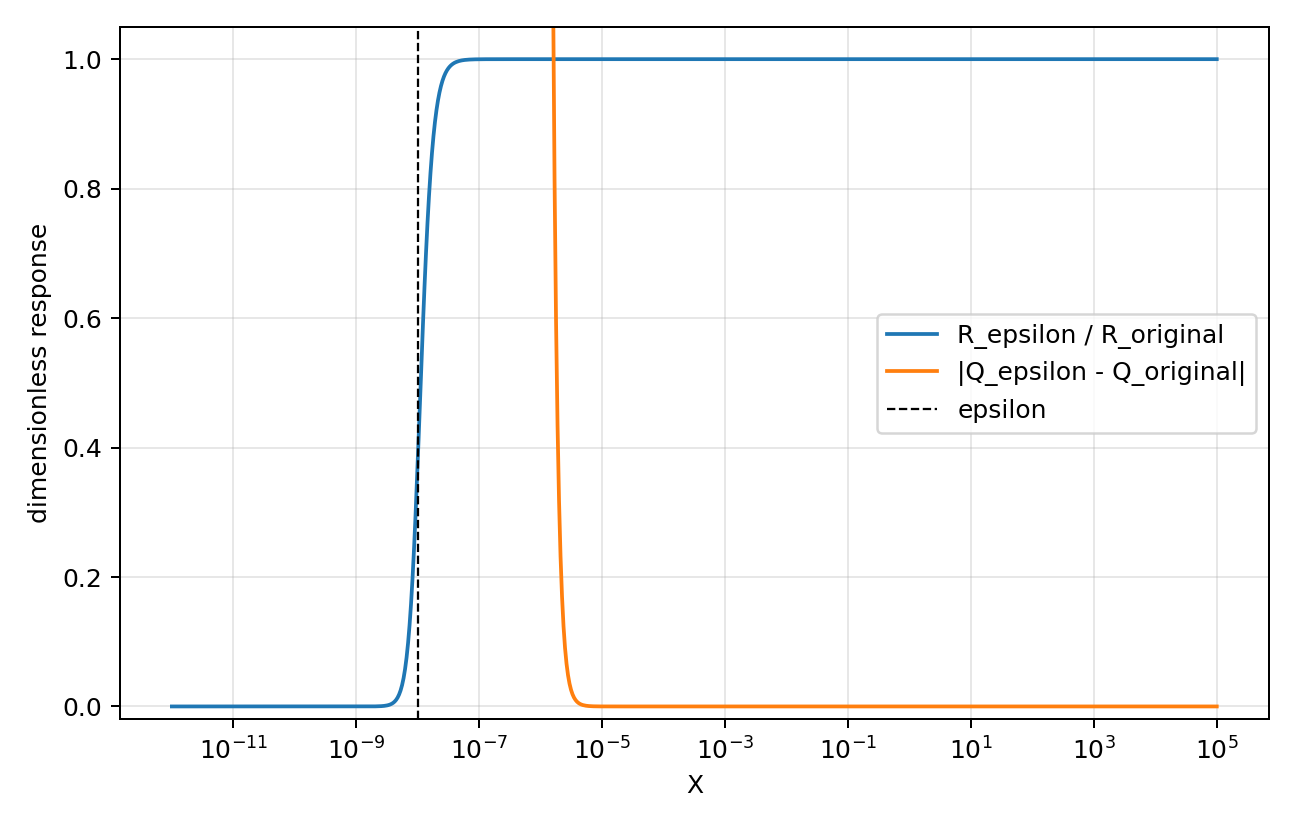
\includegraphics[draft=false,width=0.82\linewidth]{r_universe_completion/generated/figures/regularization_recovery.png}
\caption{RFG-R regularization check. The response ratio
\(\mathcal R_\epsilon/\mathcal R_{\rm original}\) and the tensor-normalization
difference \(\lvert Q_\epsilon-Q_{\rm original}\rvert\) are evaluated with
\(p=4\), \(\epsilon=10^{-8}\), and \(\theta=1.6\). Above the regulated
\(X\simeq\epsilon\) domain, RFG-R recovers the original cosmological branch;
the corresponding analytic error is given in Eq.~\eqref{eq:RFGR-recovery}.
This is an internal action-level validation, not an observational fit. Source:
\texttt{r\_universe\_completion/scripts/generate\_outputs.py}.}
\label{fig:RFGR-recovery}
\end{figure}

\begin{figure}[H]
\centering
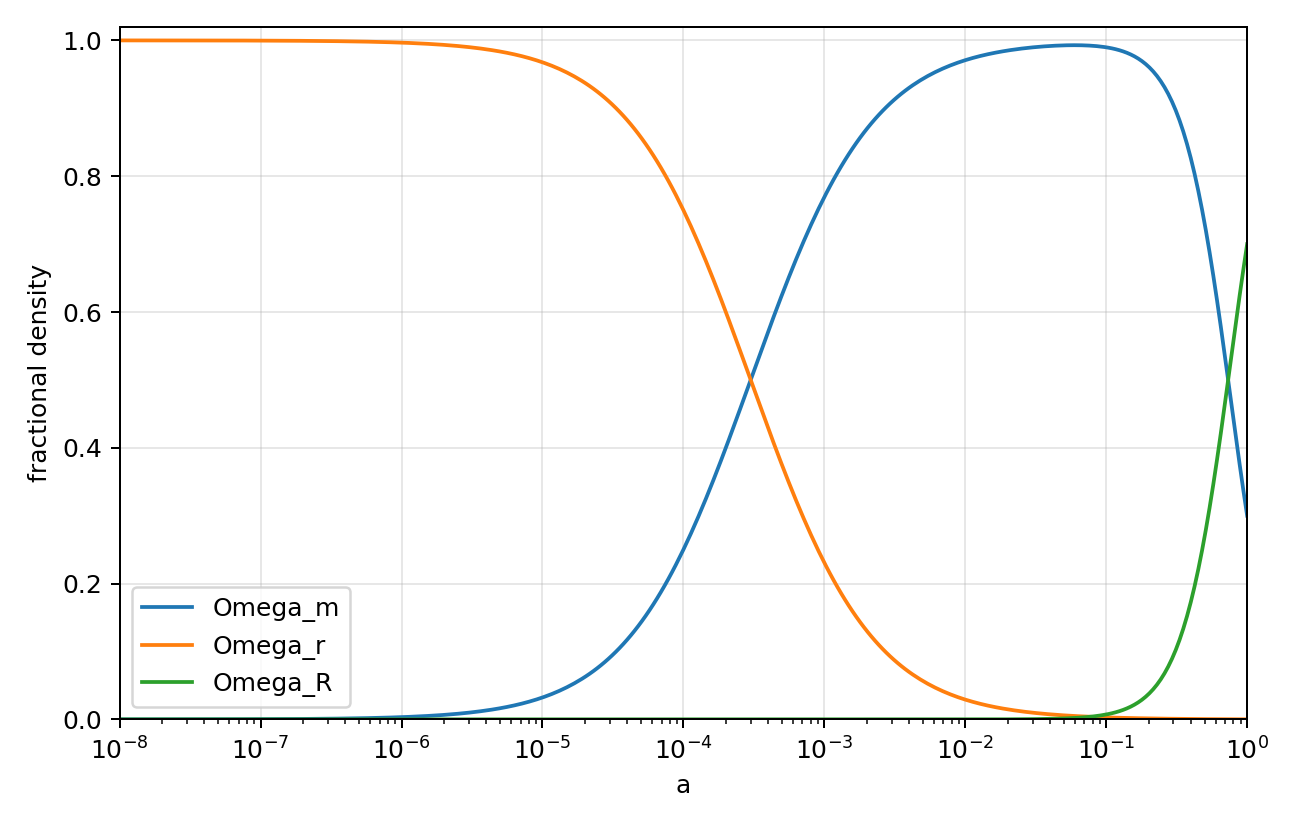
\includegraphics[draft=false,width=0.82\linewidth]{r_universe_completion/generated/figures/fractional_densities.png}
\caption{Fractional densities on the regularized RFG-R expanding branch of
Eq.~\eqref{eq:RFGR-background}, with
\(\Omega_{m0}=0.30\), \(\Omega_{r0}=9\times10^{-5}\),
\(\Omega_{R0}=0.69991\), \(\theta=1.6\), \(p=4\), and
\(\epsilon=10^{-8}\). The plot shows radiation, matter, and relational
components. It is generated from the action-reconstructed background equation;
it is not a compressed CMB constraint. Source:
\texttt{r\_universe\_completion/scripts/generate\_outputs.py}.}
\label{fig:RFGR-fractions}
\end{figure}

\begin{figure}[H]
\centering
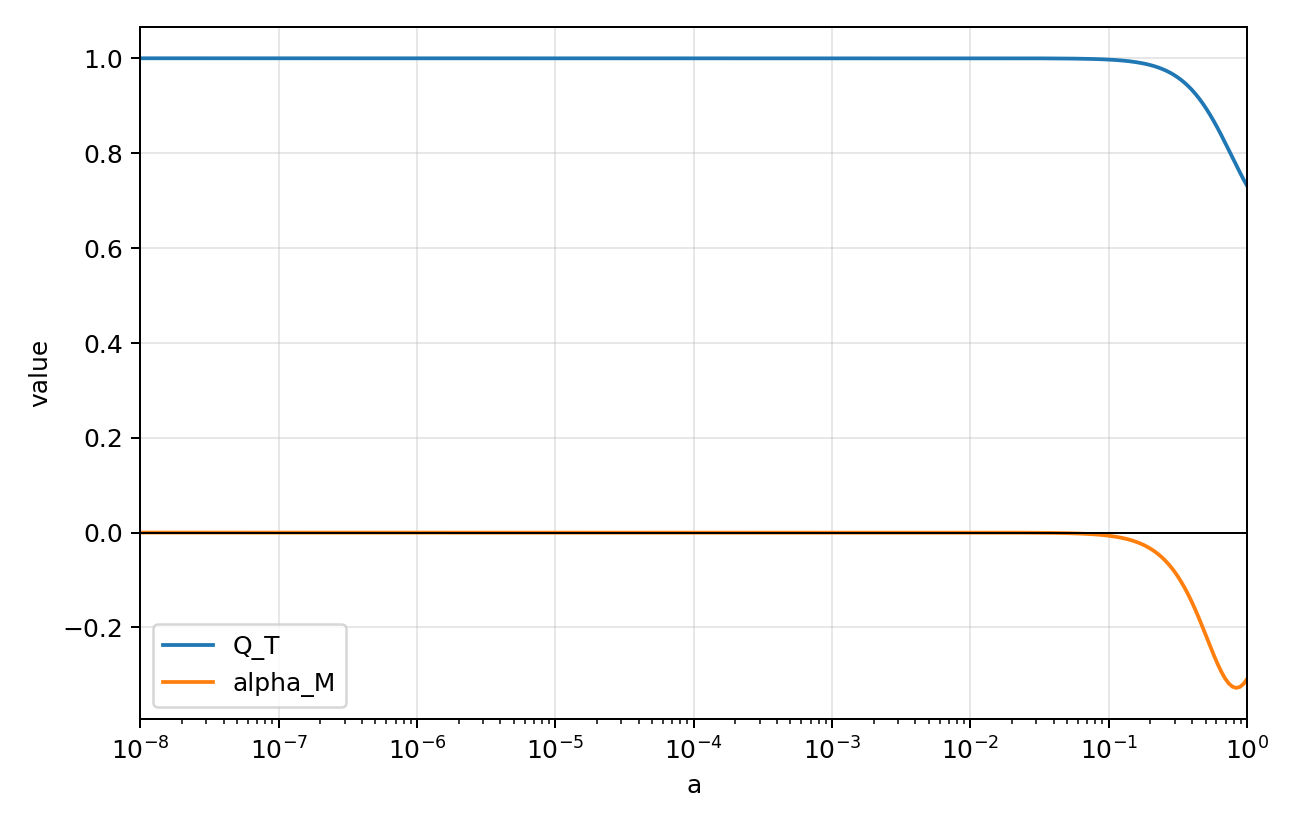
\includegraphics[draft=false,width=0.82\linewidth]{r_universe_completion/generated/figures/tensor_and_planck_running.png}
\caption{RFG-R tensor kinetic normalization \(Q_T\) and its Planck-mass
running \(\alpha_M\) as functions of scale factor on the reference branch.
The positive \(Q_T\) curve is the tensor no-ghost check behind
Eq.~\eqref{eq:RFGR-siren}; \(c_T=1\) exactly. The figure defines a
standard-siren prediction but does not itself constitute a gravitational-wave
or CMB likelihood evaluation. Source:
\texttt{r\_universe\_completion/scripts/generate\_outputs.py}.}
\label{fig:RFGR-tensor}
\end{figure}
